\documentclass[12pt]{amsart}
\setlength{\marginparwidth}{0.5in}
\usepackage{amsmath,amssymb,natbib,graphicx}
\textheight 9in
\textwidth 6.5 in
\hoffset -1 in
\voffset -1 in
\input FJHDef.tex

\newcommand{\sphere}{\mathbb{S}}
\newcommand{\cc}{\mathcal{C}}
\newcommand{\cq}{\mathcal{Q}}
\newcommand{\bbW}{\mathbb{W}}
\newcommand{\tP}{\widetilde{P}}
\newcommand{\bg}{{\bf g}}
\newcommand{\bu}{{\bf u}}
\newcommand{\bbu}{\bar{\bf u}}
\newcommand{\bv}{{\bf v}}
\newcommand{\bbv}{\bar{\bf v}}
\newcommand{\bw}{{\bf w}}
\newcommand{\bbw}{\bar{\bf w}}
\newcommand{\hv}{\hat{v}}
\DeclareMathOperator{\MSE}{MSE}
\DeclareMathOperator{\RMSE}{RMSE}
\DeclareMathOperator{\rnd}{rnd}
\DeclareMathOperator{\abso}{abs}
\DeclareMathOperator{\rel}{rel}
\DeclareMathOperator{\nor}{nor}
\DeclareMathOperator{\err}{err}
\DeclareMathOperator{\prob}{prob}
\DeclareMathOperator{\third}{third}
%\DeclareMathOperator{\fourth}{fourth}
\newtheorem{theorem}{Theorem}
\newtheorem{prop}[theorem]{Proposition}
\DeclareMathOperator{\sMC}{sMC}
\DeclareMathOperator{\aMC}{aMC}
\begin{document}

\title{Adaptive Simple Monte Carlo}
\author{Fred J. Hickernell}
\author{Lan Jiang}
\author{Yuewei Liu}
\address{Room E1-208, Department of Applied Mathematics, Illinois Institute of Technology, 10 W.\ 32$^{\text{nd}}$ St., Chicago, IL 60616}
\address{Room E1-208, Department of Applied Mathematics, Illinois Institute of Technology, 10 W.\ 32$^{\text{nd}}$ St., Chicago, IL 60616}
\address{School of Mathematics and Statistics, Lanzhou University, Lanzhou City, Gansu, China 730000}
\begin{abstract}We attempt a probabilistic analysis of simple Monte Carlo, achieving probabilistic error bounds when the kurtosis is controlled.  The algorithm uses a sample size that depends adaptively on the estimated variance of the integrand.  Thus, the algorithm is nonlinear (depending essentially on the function).  The advantage of what is done here over standard error analysis (complexity theory) is that the algorithm does not depend a priori on the scale of the problem (in this case the variance) to determine the number of samples.   Our intention, if what is done here is correct, is to try to extend this to the more sophisticated sampling schemes and infinite dimensional problems.
\end{abstract}
\maketitle

\section{Simple Monte Carlo}
Suppose one wishes to compute the following integral or mean, $\mu$, of some function $f: \reals^d \to \reals$, i.e.,
\begin{equation*}
\mu= \mu(f) = \int_{\reals^d} f(\vx) \rho(\vx) \, \dif \vx,
\end{equation*}
where $\rho: \reals^d \to [0,\infty)$ is a probability density function.  A simple Monte Carlo algorithm to estimate this integral is to generate $\vX_1, \vX_2, \ldots$ independent and identically distributed random variables with the probability density function $\rho$, i.e., $\vX_1, \vX_2, \ldots$ i.i.d.\ $\sim \rho$, evaluate the integrand at these sample points, and then take the sample mean:
\begin{equation} \label{simpleMCest}
\hmu_n = \frac 1n \sum_{i=1}^n Y_i, \qquad Y_i = f(\vX_i).
\end{equation}
This is an unbiased estimate, i.e., $E(\hmu_n) = \mu$.  Thus, the mean square error is the variance of $\hmu_n$:
\begin{equation}\label{MSE1}
\MSE(\hmu_n) = E[(\mu-\hmu_n)^2]=\var(\hmu_n) = \frac{\var(Y_1)}{n}.
\end{equation}

The variance of $Y_1$ may be written in terms of an integral of the $f$.  Define the $\cl_{p}$ norm of $f$ as follows:
\[
\norm[p]{f} :=\left\{\int_{\reals^d} \abs{f(\vx)}^p \rho(\vx) \, \dif \vx\right\}^{1/p}
\]
Note that if $1 \le q<p$, then by H\"older's inequality,
\begin{align}\label{LP}
\norm[q]{f} &=\left\{\int_{\reals^d} \abs{f(\vx)}^q \rho(\vx) \, \dif \vx\right\}^{1/q}\\
\nonumber & \le \left\{\int_{\reals^d} \abs{f(\vx)}^p f(\vx) \, \dif \vx \right\}^{1/p} \left\{\int_{\reals^d} 1^{p/(p-q)} f(\vx) \, \dif \vx\right\}^{(p-q)/(pq)} \\
\nonumber & = \norm[p]{f} \norm[pq/(p-q)]{1} = \norm[p]{f}.
\end{align}
Thus, $\cl_q \subseteq \cl_p$ for $1 \le q<p$.  

Now define the the centered absolute $p^{\text{th}}$ moment of $f$ as
\begin{equation} \label{momentdef}
M_p(f) := \int_{\reals^d} \abs{f(\vx)-\mu}^p \rho(\vx) \, \dif \vx, \qquad p \ge 1
\end{equation}
By this definition, the variance of $Y_1$ is the second moment, i.e., 
\begin{equation} \label{sigmadef}
\sigma^2 := \var(Y_1) = \var(f(\vX_1)) =: \var(f) = M_2(f) = \int_{\reals^d} \abs{f(\vx)-\mu}^2 \rho(\vx) \, \dif \vx.
\end{equation}
Moreover, by \eqref{LP} it follows that low order moments can be bounded above by higher order moments.
\begin{equation}\label{Mineq}
M_q \le M_p^{q/p} \quad \text{and} \quad M_p < \infty \implies M_q <\infty \qquad \text{for }1 \le q \le p.
\end{equation}
Thus, the root mean square error of the simple Monte Carlo quadrature rule, given in \eqref{MSE1}, may be written in terms of the second moment of $f$ as
\begin{equation}\label{MSE2}
\RMSE(\hmu_n) = \frac{\sigma}{\sqrt{n}} = \sqrt{\frac{\var(f)}{n}}.
\end{equation}

\section{Randomized Error Analysis}

Given an error tolerance, $\varepsilon$, and a set of functions, $\cf$, one may ask how large a sample size is needed to guarantee that this tolerance is achieved.  The answer depends on the error criterion.  Here are three possibilities defined for our simple Monte Carlo (sMC) algorithm:
\begin{subequations} \label{randerrcrit}
\begin{align}
\text{randomized absolute} \quad & 
\err^{\rnd\abso}(n,\cf,\sMC) := \sup_{f \in \cf} \RMSE(\hmu_n) =  \sqrt{\frac{\sup_{f \in \cf}\var(f)}{n}},\\
\text{randomized relative} \quad & 
\err^{\rnd\rel}(n,\cf,\sMC) := \sup_{f \in \cf} \frac{\RMSE(\hmu_n)} {\mu}=  \frac{1}{\sqrt{n}} \sup_{f \in \cf} \frac{\sqrt{\var(f)}}{\mu(f)} , \\
\text{randomized normalized} \quad & 
\err^{\rnd\nor}(n,\cf,\sMC) := \sup_{f \in \cf} \frac{\RMSE(\hmu_n)} {\sqrt{\var(f)}} =  \frac{1}{\sqrt{n}}.
\end{align}
\end{subequations}
Here the root mean square error is taken over all $\hmu_n$ with cardinality $n$.  Given an error criterion, $\err^{\text{x}}$, the sample size needed to attain the error tolerance, $\varepsilon$. for this class of algorithms with deterministic sample size is defined as 
\[
\cost^{\text{x}}(\varepsilon,\cf,\sMC) = \min \{{n \in \natzero} :  \err^{\text{x}}(n,\cf,\sMC) \le \varepsilon\},
\]
where $\text{x} \in \{\rnd\abso, \rnd\rel, \rnd\nor\}$.
For the error criteria in \eqref{randerrcrit} and the simple Monte Carlo algorithm, it is found that 
\begin{subequations} \label{randerrcritsample}
\begin{align}
\cost^{\rnd\abso}(\varepsilon,\cf^{\abso},\sMC) &= \frac{\sigma^2_{\max}} {\varepsilon^2}, & \cf^{\abso} &= \left\{f \in \cl_2 : \var(f) \le \sigma^2_{\max} \right\},\\
\cost^{\rnd\rel}(\varepsilon,\cf^{\rel},\sMC) & = \frac{a^2} {\varepsilon^2}, & \cf^{\rel} &= \left\{f \in \cl_2 : \frac{\var(f)}{[\mu(f)]^2} \le a^2,\ \mu(f) \ne 0 \right\}, \\
\cost^{\rnd\nor}(\varepsilon,\cf^{\nor},\sMC) & = \frac{1} {\varepsilon^2}, & \cf^{\nor} &= \cl_2.
\end{align}
\end{subequations}

The error analyses above have some practical shortcomings.  To apply the randomized absolute case one must have some a priori knowledge of the variance of the integrand.  It must not larger than $\sigma^2_{\max}$ or the theory does not apply.  If the variance of the integrand is much smaller than $\sigma^2_{\max}$, then the specified sample size, $\cost^{\rnd\abso}(\varepsilon,\cf^{\abso},\sMC)$ is much too large. The randomized relative case is even more problematic since determining whether $f \in \cf^{\rel}$ requires a priori knowledge of the ratio of the variance of the integrand to its squared mean.  The randomized normalized case avoids the problem of requiring a priori knowledge of the integrand variance by including the variance of the integrand in the error criterion.  However, still this does not give the practioner a clear idea of how large the error will be, only that it can be made small relative to the squre root of the variance of the integrand.

\section{Probabilistic Error Analysis}

Another approach that appears somewhat more stringent than the randomized error setting is the probabilistic error setting.  In this case one wishes to be $(1-\alpha)100\%$ certain of achieving an error tolerance.  Again there may be different cases:
\begin{subequations} \label{proberrcrit}
\begin{multline}
\text{probabilistic absolute} \\ 
\err^{\prob\abso}(n,\alpha,\cf,\sMC) := \min \left \{\varepsilon :  \sup_{f \in \cf} \Prob\left[\abs{\hmu_n-\mu} \le \varepsilon \right] \ge 1-\alpha \right \},
\end{multline}
\begin{multline}
\text{probabilistic relative} \\ 
\err^{\prob\rel}(n,\alpha,\cf,\sMC) := \min \left \{\varepsilon :  \sup_{f \in \cf} \Prob\left[\abs{\frac{\hmu_n-\mu}{\mu}} \le \varepsilon \right] \ge 1-\alpha \right \},
\end{multline}
\begin{multline}
\text{probabilistic normalized} \\ 
\err^{\prob\nor}(n,\alpha,\cf,\sMC) := \min \left \{\varepsilon :  \sup_{f \in \cf} \Prob\left[\abs{\frac{\hmu_n-\mu}{\sigma}} \le \varepsilon \right] \ge 1-\alpha \right \},
\end{multline}
\end{subequations}
Again one may define the minimum number of function values required to attain a given error tolerance as
\[
\cost^{\text{x}}(\varepsilon,\alpha,\cf,\sMC) = \min \{{n \in \natzero} :  \err^{\text{x}}(n,\alpha,\cf,\sMC) \le \varepsilon\},
\]
where $\text{x} \in \{\prob\abso, \prob\rel, \prob\nor\}$.

These error measures also have the practical shortcomings as described for the randomized error analysis.  However, we will find ways to overcome them.


In practice, one often invokes the Central Limit Theorem to determine sample size. Given a significance level or uncertainty tolerance, $\alpha$, one has
\[
\Prob\left[\abs{\hmu_n-\mu} \le \frac{z_{\alpha/2} \sigma}{\sqrt{n}} \right] \approx 1-\alpha.
\]
This directly leads to  the \emph{approximate} probabilistic result:
\begin{subequations} \label{proberrcritsampleGauss}
\begin{align}
\cost^{\prob\abso}(\varepsilon,\cf^{\abso},\sMC) &\approx  N_{G}(\varepsilon/\sigma_{\max},\alpha), & \text{where } N_{G}(\varepsilon,\alpha) :=\left \lceil \left(\frac{z_{\alpha/2}}{\varepsilon}\right)^2 \right \rceil,\\
\cost^{\prob\rel}(\varepsilon,\cf^{\rel},\sMC) & \approx  N_{G}(\varepsilon/a,\alpha), \\
\cost^{\prob\nor}(\varepsilon,\cf^{\nor},\sMC) &\approx  N_{G}(\varepsilon,\alpha).
\end{align}
\end{subequations}
The above is exact if the $Y_i=f(\vX_i)$ are i.i.d.\ Gaussian, however, in general this result is only approximate.

Using Chebyshev's inequality (Theorem \ref{Chebineqthm}) yields an exact upper bound rather than approximate one.  Choosing $Z=\hmu_n$ yields
\[
\Prob\left[\abs{\hmu_n-\mu} < \frac{\sigma}{\sqrt{n \alpha}} \right] \ge 1-\alpha.
\]
This inequality leads to an \emph{upper bound} on the sample size required to guarantee that the estimated mean is within the tolerance of the true answer with probability $1-\alpha$:
\begin{subequations} \label{proberrcritsampleCheby}
\begin{align}
\cost^{\prob\abso}(\varepsilon,\cf^{\abso},\sMC) &\le N_{C}(\varepsilon/\sigma_{\max},\alpha), & \text{where }N_{C}(\varepsilon,\alpha) :=\left \lceil \frac{1}{\alpha\varepsilon^2} \right \rceil,\\
\cost^{\prob\rel}(\varepsilon,\cf^{\rel},\sMC) & \le N_{C}(\varepsilon/a,\alpha), \\
\cost^{\prob\nor}(\varepsilon,\cf^{\nor},\sMC) &\le N_{C}(\varepsilon,\alpha).
\end{align}
\end{subequations}
The sample size $N_C$ is typically much larger than $ N_G$, since $1/\alpha$ is much larger than $z_{\alpha/2}^2$ as $\alpha \to 0$.  Figure \ref{alphacomparefig} compares these two quantities.

\begin{figure}
\centering
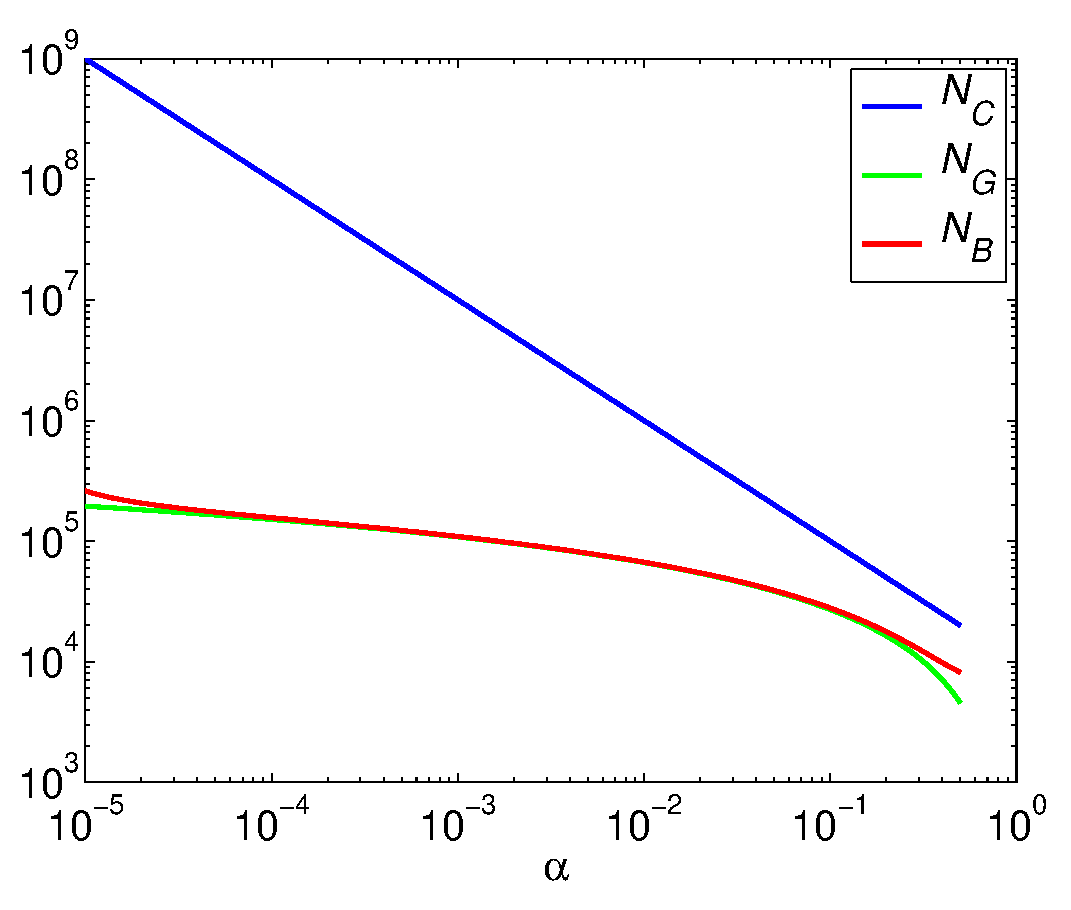
\includegraphics[width=3in]{alphacompare.eps} \quad 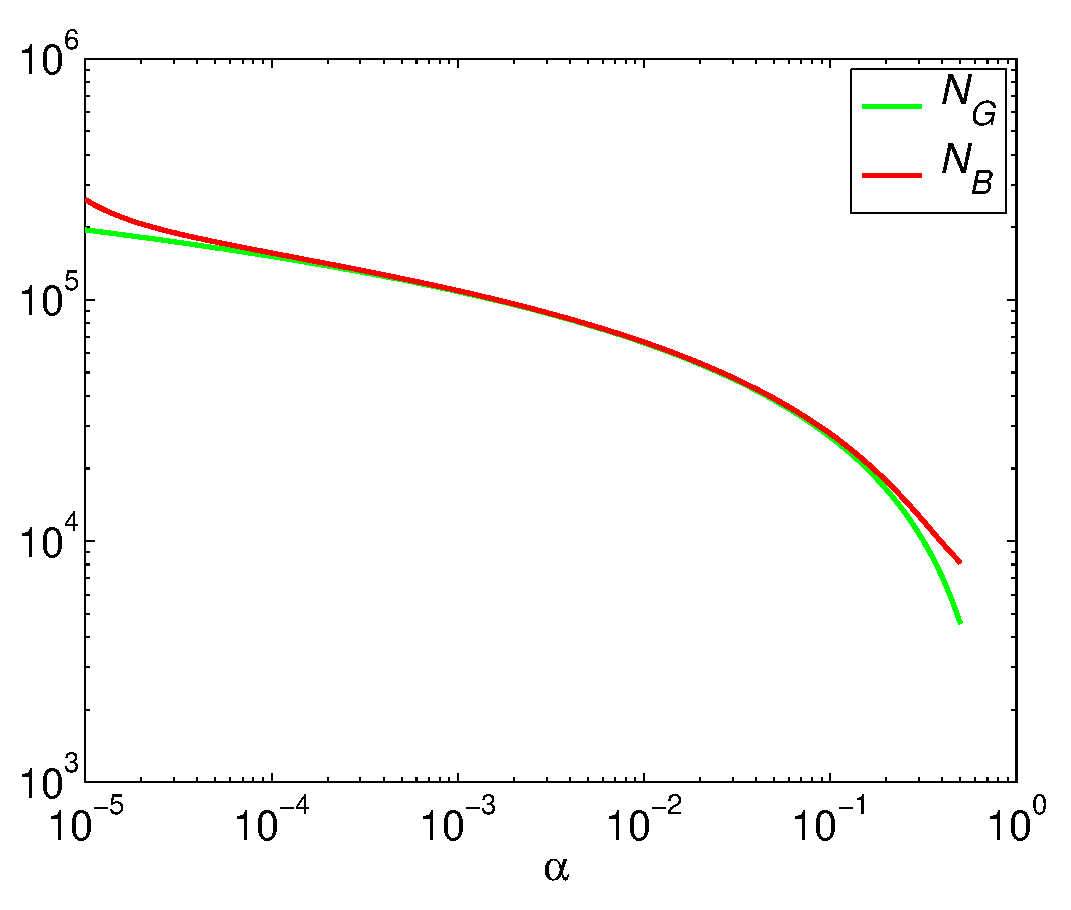
\includegraphics[width=3in]{alphacompareb.eps} \quad 
\caption{Comparison of $ N_G(\varepsilon,\alpha)$, $N_C(\varepsilon,\alpha)$, and $N_B(\varepsilon,\alpha,\varrho)$ for $\varepsilon = 0.001$, and $\varrho=5$. \label{alphacomparefig}}
\end{figure}

A smaller sample size with a rigorous probabilistic bound can be
found by invoking the non-uniform Berry-Esseen inequality (Theorem
\ref{BE}). This inequality makes strong assumptions on the
distribution of $f(\vX)$, namely, a finite third moment:
\[
\varrho:=\frac{M_3}{\sigma^3} < \infty.
\]
However, this assumption is weaker than the one that we intend to make below to justify the approximation of the variance by its sample quantity.  Recalling that $Y_i = g(\vX_i)$, $\mu=E(Y_i)$, and $\hmu_n =
(Y_1 + \cdots + Y_n)/n$, it then follows by the non-uniform
Berry-Esseen inequality,
\begin{align*}
\Prob\left[\abs{\hmu_n - \mu} <\frac{\sigma}{\sqrt{n}}x\right]&=\Prob\left[\hmu_n - \mu<\frac{\sigma}{\sqrt{n}}x\right]-\Prob\left[\hmu_n - \mu <-\frac{\sigma}{\sqrt{n}}x\right]\\
&\ge \left[\Phi(x)-A\frac{\varrho}{\sqrt{n}}(1+\abs{x})^{-3}\right] -\left[\Phi(-x) + A\frac{\varrho}{\sqrt{n}}(1+\abs{x})^{-3}\right]\\
&=1-2\left(A\frac{\varrho}{\sqrt{n}}(1+\abs{x})^{-3}+\Phi(-x)\right).
\end{align*}
Letting $b=x/\sqrt{n}$, the probability of
making a small error becomes 
\[
\Prob[\abs{\hmu_n -
\mu}<b \sigma] \geq
1-2\left(A\frac{\varrho}{\sqrt{n}}\left(1+b\sqrt{n}\right)^{-3}+\Phi\left(-b\sqrt{n}\right)\right)\geq
1-\alpha,
\]
provided that $n$ is chosen to be larger than
\begin{equation}\label{NB}
N_B(b,\alpha,\varrho) := \min \left \{ n \in \naturals : \Phi\left(-b \sqrt{n}  \right)+\frac{A\varrho}{\sqrt{n}}\left(1+ b\sqrt{n} \right)^{-3}
\le \frac{\alpha}{2} \right \}.
\end{equation}

This inequality leads to an \emph{upper bound} on the work required to meet the probabilistic error criterion, but this time for a smaller set of functions.  guarantee that the estimated mean is within the tolerance of the true answer with probability $1-\alpha$:
\begin{subequations} \label{proberrcritsampleBE}
\begin{align}
\cost^{\prob\abso}(\varepsilon,\cf^{\abso} \cap \cf^{\third},\sMC) &\le N_{B}(\varepsilon/\sigma_{\max},\alpha,\varrho_{\max}), \\
\cost^{\prob\rel}(\varepsilon,\cf^{\rel}\cap \cf^{\third},\sMC) & \le N_{B}(\varepsilon/a,\alpha,\varrho_{\max}), \\
\cost^{\prob\nor}(\varepsilon,\cf^{\nor}\cap \cf^{\third},\sMC) &\le N_{B}(\varepsilon,\alpha,\varrho_{\max}),
\intertext{where}
\cf^{\third}& :=\left \{ f \in \cl_3 : \frac{M_3(f)}{[\var(f)]^{3/2}} \le \rho_{\max} \right \}.
\end{align}
\end{subequations}

Definition \eqref{NB} may be re-written implicitly
\begin{equation}\label{NBalt}
N_B = \left \lceil \left(\frac{z_{\alpha/2 -  A
\varrho/(\sqrt{N_B}(1+b\sqrt{N_B})^3)}}{b}\right)^2 \right \rceil.
\end{equation}
The definition of $N_B$ implies that
\[
N_G(b,\alpha) \le N_B(b,\alpha,\varrho) \le \min_{0 \le
\theta \le 1} \left\{\max\left[ \sqrt{\frac{2A
\rho}{\theta\alpha b^3}},
 N_G(b,(1-\theta)\alpha)  \right] \right\}.
\]
As shown in Figure \ref{alphacomparefig}, $N_B$ is close to $ N_G$ for moderate $\alpha$, but $N_B$ may be significantly larger for very small $\alpha$.

\section{Adaptive Monte Carlo}
The Chebyshev and the Berry-Esseen inequalities provide upper bounds on the sample size required by the simple Monte Carlo algorithm to attain the desired error tolerance under the probabilistic error criterion, \eqref{proberrcritsampleCheby} and \eqref{proberrcritsampleBE}, respectively.  However, as mentioned earlier, in the case of the absolute and relative error criterion, the classes of integrands are defined in terms of quantities, such as $\sigma^2=\var(f)$, which are typically unknown.  For the case of normalized error, the error criterion is defined in terms of $\var(f)$.  

In practice one typically uses observed function values observed to approximate $\sigma^2$ by the sample variance, as follows:
\begin{equation} \label{samplevar}
\hv_{n} = \frac 1{n-1} \sum_{i=1}^{n} [f(\vX_i)- \hmu_{n}]^2.
\end{equation}
This means that we now have an \emph{adaptive} algorithm.  One might choose an initial sample of size $n_0$, and use it to estimate $\sigma^2$ by $\hv_{n_0}$.  Then one chooses an \emph{independent} sample of size $n=N_{C}(\varepsilon/\sqrt{\hv_{n_0}},\alpha)$, or  $n=N_{B}(\varepsilon/\sqrt{\hv_{n_0}},\alpha,\varrho_{\max})$ to compute $\hmu_n$ the final estimate of $\mu$.

Unfortunately, once we approximate $\sigma^2$ by $\hv_n$, we again have inexact results.  However, they can be made exact by using Cantelli's inequality (Theorem \ref{Can}) and the variance of $\hv_n$ in Theorem \ref{Varvarthm}.  Proposition \ref{propCant} implies that
\[
\Prob\left[\frac{\hv_n}{1 - \sqrt{\left ( \kappa  - \frac{n-3}{n-1}\right)\left(\frac{1-\alpha}{\alpha n}\right)}} > \sigma^2 \right] \ge 1 - \alpha,
\]
where
\begin{equation} \label{kurtdef}
\kappa:= \kurt(f) = \frac{M_4(f)}{\var^2(f)} = \frac{M_4(f)}{\sigma^4(f)} \ge 1 \qquad \forall f \in \cl_4
\end{equation}
denotes the \emph{kurtosis}.  Note that the kurtosis of a function is independent of scale.  Thus, it follows that
\begin{subequations}\label{probvarupbd}
\begin{gather}
\Prob\left[\hsigma_{\text{up}}(\hv_n,n,\alpha,\kappa)  > \sigma \right] \ge 1 - \alpha, \\
\text{where } \hsigma^2_{\text{up}}(\hv_n,n,\alpha,\kappa) = \frac{\hv_{n}}{1 - \sqrt{ \left ( \kappa  - \frac{n-3}{n-1}\right)\left(\frac{1-\alpha}{\alpha n }\right)}},
\end{gather}
\end{subequations}
provided that
\begin{align*}
1 &> \left ( \kappa  - \frac{n-3}{n-1}\right)\left(\frac{1-\alpha}{ \alpha n}\right)\\
\frac{\alpha n }{1-\alpha} & > \kappa  - \frac{n-3}{n-1} \\
\kappa & < \frac{\alpha n}{1-\alpha} + \frac{n-3}{n-1} =: \kappa_{\text{poss}} (\alpha,n).
\end{align*}

From another perspective, if we want the amplification factor to be smaller than $L$, i.e.,
\[
\frac{1}{1 - \sqrt{ \left ( \kappa  - \frac{n-3}{n-1}\right)\left(\frac{1-\alpha}{\alpha n }\right)}} \le L,
\]
then $n$ must be chosen to satisfy
\begin{gather*}
\left(\kappa  - \frac{n-3}{n-1}\right)\left(\frac{1-\alpha}{\alpha n }\right) \le \frac{L-1}{L}, \\
M\left[(\kappa-1)  + \frac{2}{n-1}\right] \le n, \qquad \text{where } M= \left(\frac{1-\alpha}{\alpha}\right)  \left(\frac{L}{L-1} \right), \\
(n-1)^2 - [(\kappa-1)M -1](n-1)  - 2 M \ge 0, \\
n \ge 1 + \frac{1}{2} \left\{ (\kappa-1)M -1 + \sqrt{\left[(\kappa-1)M -1\right]^2 + 8 M}\right\}.
\end{gather*}
Thus, for example, even in the best case scenario of $\kappa=1$, the smallest possible value, we have $n \ge [1 + \sqrt{1 + 8 M}]/2$.  For $L=2$ and $\alpha=0.05$ this translates into $M=38$ and $n \ge 9.2$.

On the other hand, suppose that we choose
\[
\hsigma^2_{\text{up}} = L \hv_{n}
\]
where $L$ is a \emph{fudge factor}.  This means that we are implicitly assuming the kurtosis to satisfy
\begin{align*}
\frac{1}
{1 - \sqrt{ \left ( \kappa  - \frac{n-3}{n-1}\right)\left(\frac{1-\alpha}{\alpha n }\right)}} &\le L, \\
\frac{1}{L} &\le 1 - \sqrt{ \left ( \kappa  - \frac{n-3}{n-1}\right)\left(\frac{1-\alpha}{\alpha n }\right)}, \\
\left ( \kappa  - \frac{n-3}{n-1}\right)\left(\frac{1-\alpha}{\alpha n }\right) &\le \left(1 - \frac{1}{L}\right)^2 = \left(\frac{L-1}{L}\right)^2,\\
\kappa  & \le \frac{n-3}{n-1} + \left(\frac{1-\alpha}{\alpha n }\right)\left(\frac{L-1}{L}\right)^2.
\end{align*}

From still another perspective, for a given $n$ and $\kappa$, one must require $\alpha$ large enough, namely
\begin{gather*}
\frac{1}{ n }\left(\kappa  - \frac{n-3}{n-1}\right)\left(\frac{1-\alpha}{\alpha}\right) < 1, \\
\alpha>\frac{1}{1+\frac{n}{\kappa  - \frac{n-3}{n-1}}}.
\end{gather*}
Figure  \ref{ampfacfig} shows how much the sample variance needs to be inflated to be confident that the true variance is not underestimated. Notice that for $n=30$, the common rule of thumb for applying the central limit theorem, even $\alpha=0.1$ is not possible.

\begin{figure}
\centering
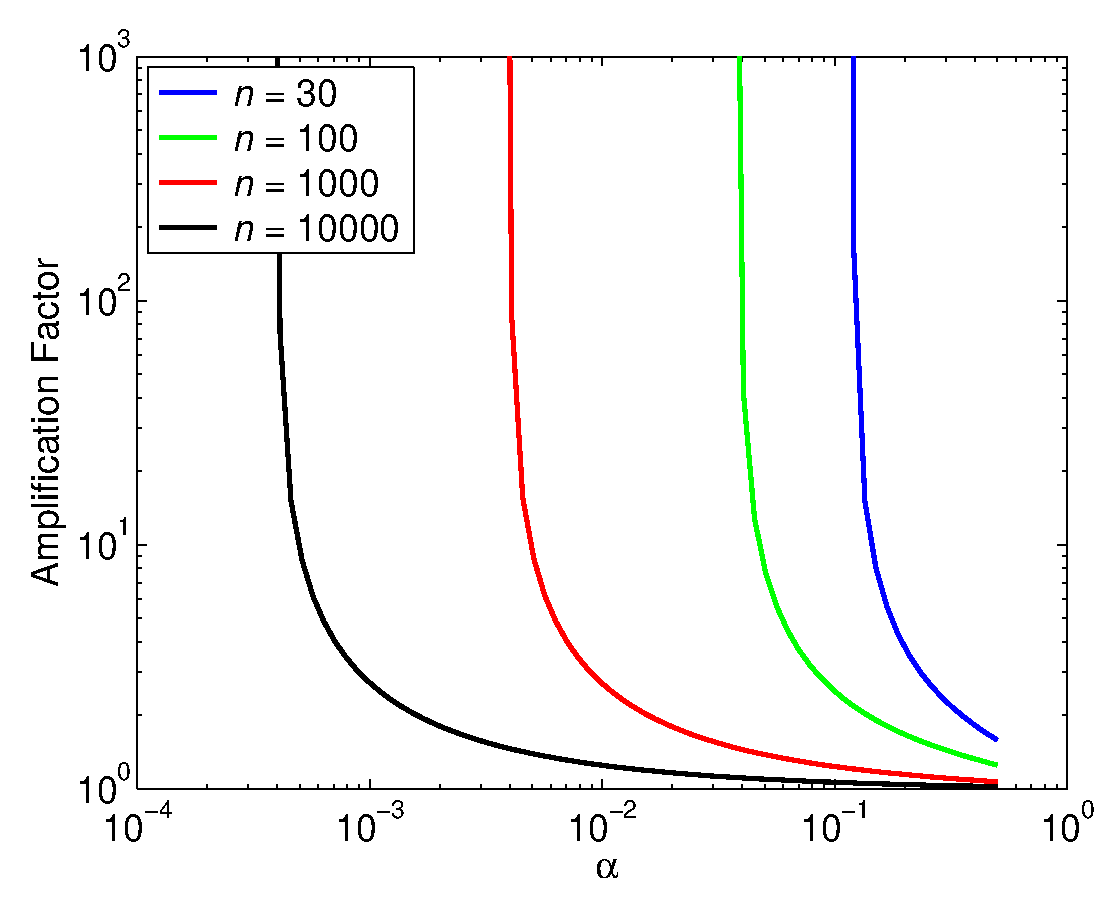
\includegraphics[width=3in]{varianceampfac.eps}
\caption{The amplification factor, $\hsigma^2_{\text{up}}/\sigma^2$, as a function of $\alpha$ for various $n$ and for $\kappa=5$. \label{ampfacfig}}
\end{figure}


\begin{theorem} \label{mainadaptthm} For a given positive constant, $\kappa_{\max}$, define the set of functions with bounded fourth moments:
\[
\cf^{\kurt}= \{f \in \cl_{4} : \kurt(f)= \kappa \le \kappa_{\max} \},
\]
where the kurtosis of the function is defined in \eqref{kurtdef}.
Suppose that one has an error tolerance, $\varepsilon$, and an uncertainty tolerance, $\alpha$. Let $\alpha_1 = 1 - \sqrt{1 - \alpha}$.  Pick any $n_0>1$ satisfying
\[
\kappa_{\max} < \kappa_{\text{\rm poss}}(\alpha_1,n_0)  = \frac{n_0 \alpha_1}{1-\alpha_1} + \frac{n_0-3}{n_0-1},
\]
and compute the sample variance, $\hv_{n_0}$ of a simple random sample of size $n_0$.   Use this to compute $\hsigma^2_{\text{\rm up}} = \hsigma^2_{\text{\rm up}}(\hv_{n_0},n_0,\alpha_1,\kappa_{\max})$ by \eqref{probvarupbd}.  Next choose an independent random sample of size
\[
n = \min\left( N_C(\varepsilon/\hsigma_{\text{\rm up}},\alpha_1), N_B(\varepsilon/\hsigma_{\text{\rm up}},\alpha_1,\kappa_{\max}^{3/4}) \right)
\]
and compute $\hmu_n$, the simple Monte Carlo estimator of $\mu$.  Here $N_C$ is defined in \eqref{proberrcritsampleCheby} and  $N_B$ is defined in \eqref{NB}.  A probabilistic error bound is given by
\[
\Prob\left[\abs{\hmu_n-\mu} \le \epsilon \right] \geq 1-\alpha.
\]
\end{theorem}
\begin{proof}
By \eqref{probvarupbd} it follows that $\hsigma_{\text{up}}(\hv_{n_0},n_0,\alpha_1,\kappa)  \ge \sigma$ with probability $1-\alpha_1$.  By  \eqref{proberrcritsampleCheby} and \eqref{proberrcritsampleBE} it follows that  $\Prob\left[\abs{\hmu_n-\mu} \le \epsilon \right] \geq 1-\alpha_1$, provided that $\hsigma_{\text{up}}  \ge \sigma$.  Thus, the probability that both of these events happen, is at least $(1-\alpha_1)^2=1-\alpha$.
\end{proof}

The sample size of this algorithm is now a random variable, and so the cost is defined probabilistically.  Define the cost of an algorithm as the $1-\beta$ quantile of the total number of function evaluations.  Furthermore, the cost now depends not only on the space of functions, but also on the variance of the integrand, which is stated explicitly:
\begin{equation}
\cost(\varepsilon,\sigma^2,\cf^{\kurt},\aMC) := \sup_{\substack{f \in \cf^{\kurt}\\ \var(f)\le \sigma^2} } \min\left\{M : \Prob(n_0 + n \le M) \ge 1-\beta  \right \}.
\end{equation}

From form Proposition \ref{propCant} it follows that
\begin{align*}
1-\beta & \le \Prob\left[\hv_n < \sigma^2 \left\{1 + \sqrt{\left ( \kappa  - \frac{n-3}{n-1}\right)\left(\frac{1-\beta}{\beta n}\right)}\right\} \right] \\
& = \Prob\left[\frac{\hv_n} {1 - \sqrt{\left ( \kappa  - \frac{n-3}{n-1}\right)\left(\frac{1-\alpha_1}{\alpha_1 n}\right)}} < \sigma^2 \left\{\frac{1 + \sqrt{\left ( \kappa  - \frac{n-3}{n-1}\right)\left(\frac{1-\beta}{\beta n}\right)}} {1 - \sqrt{\left ( \kappa  - \frac{n-3}{n-1}\right)\left(\frac{1-\alpha_1}{\alpha_1 n}\right)}} \right\} \right] \\
& = \Prob\left[\hsigma^2_{\text{\rm up}}(\hv_{n},n,\alpha_1,\kappa_{\max}) < \sigma^2 \gamma^2(n,\alpha_1,\beta,\kappa_{\max}) \right],
\end{align*}
where,
\[
\gamma^2(n,\alpha_1,\beta,\kappa_{\max}) := \frac{1 + \sqrt{\left ( \kappa  - \frac{n-3}{n-1}\right)\left(\frac{1-\beta}{\beta n}\right)}} {1 - \sqrt{\left ( \kappa  - \frac{n-3}{n-1}\right)\left(\frac{1-\alpha_1}{\alpha_1 n}\right)}} > 1.
\]
Since $N_C(\cdot,\alpha_1)$ and $N_B(\cdot,\alpha_1,\kappa_{\max}^{3/4})$ are decreasing functions, it follows that
\begin{multline} \label{adaptcost}
\cost(\varepsilon,\sigma^2,\cf^{\kurt},\aMC) = \sup_{\substack{f \in \cf^{\kurt}\\ \var(f)\le \sigma^2} } \min\left\{M : \Prob(n_0 + n \le M) \ge 1-\beta  \right \}\\
= n_0 + \min\left\{M : \Prob\left( \min\left( N_C(\varepsilon/\hsigma_{\text{\rm up}},\alpha_1), N_B(\varepsilon/\hsigma_{\text{\rm up}},\alpha_1,\kappa_{\max}^{3/4}) \right) \le M\right) \ge 1-\beta  \right \}]] \\
\le n_0 + \min\left( N_C(\varepsilon/(\sigma\gamma(n_0,\alpha_1,\beta,\kappa_{\max})),\alpha_1), N_B(\varepsilon/(\sigma\gamma(n_0,\alpha_1,\beta,\kappa_{\max})),\alpha_1,\kappa_{\max}^{3/4}) \right).
\end{multline}

\begin{theorem} \label{costtheorem} The algorithm described in Theorem \ref{mainadaptthm} has a probabilistic cost given by \eqref{adaptcost}.
\end{theorem}

The key factors that determine $\cost(\varepsilon,\sigma^2,\cf^{\kurt},\aMC)$ are $\varepsilon$, the error tolerance, and $\sigma^2$, the variance of the integrand.  The cost is roughly proportional to $\sigma^2\epsilon^{-2}$.  For the set of integrands $\cf^{\kurt}$ the variance, $\var(f)$ is unbounded.  Thus, the cost is not bounded, however, it does seem to behave as expected as a function of the variance of the integrand.  As mentioned before, this is actually an advantage of this analysis.  One need not make any assumptions about the variance of the integrand, only about the kurtosis, which is unchanged when the integrand is multiplied by an arbitrary constant.

%Consider a spacial case in (\ref{NB}), let $\Phi(-\frac{\sqrt{n}\epsilon}{\sigma})=\frac{A\varrho}{\sqrt{n}}=\frac{\alpha}{4}$, since $\varrho\leq (\kappa_{\max}+3)^{3/4}$,
%we can get the upper bound of $N_B(\epsilon,\alpha_1,\sigma_{\max},\varrho)$ by
%$$N_B(\epsilon,\alpha_1,\sigma_{\max},\varrho)\leq \max\{\frac{Z^2_{\alpha_1/4}\sigma^2_{\max}}{\epsilon^2},\frac{16A^2(\kappa_{\max}+3)^{3/2}}{\epsilon^2}\}$$

\section{Example}

Consider the case of the uniform probability distribution on $[0,1]$, i.e., $\rho=1$.  Define
\begin{equation} \label{exampleeq}
f(x) = \begin{cases} 1 + \sigma \sqrt{\frac{1-p}{p}}, & 0 \le x \le p,\\
1 - \sigma \sqrt{\frac{p}{1-p}}, & p < x \le 1,
\end{cases}
\end{equation}
where $p$ and $\sigma$ are parameters, with $0 < p < 1$.
Note that
\begin{align*}
\mu &= \int_0^1 g(x) \, \dif x = 1\\
\var(g) &= \int_0^1 [g(x)-\mu]^2 \, \dif x = \sigma^2 \frac{1-p}{p} p + \sigma^2 \frac{p}{1-p} (1-p) = \sigma^2, \\
\kappa = \kurt(g) &= \frac{1}{\sigma^4}\int_0^1 [g(x)-\mu]^4 \, \dif x = \left(\frac{1-p}{p}\right)^2 p + \left(\frac{p}{1-p} \right)^2 (1-p) \\
& = \frac{(1-p)^3 + p^3}{p(1-p)} = \frac{1-3p+3p^2}{p(1-p)} = \frac{1}{p(1-p)} - 3.
\end{align*}
Note that $\kappa$ ranges from a minimum of $1$, when $p=1/2$ to a maximum of $\infty$ when $p=0,1$.

\begin{figure}
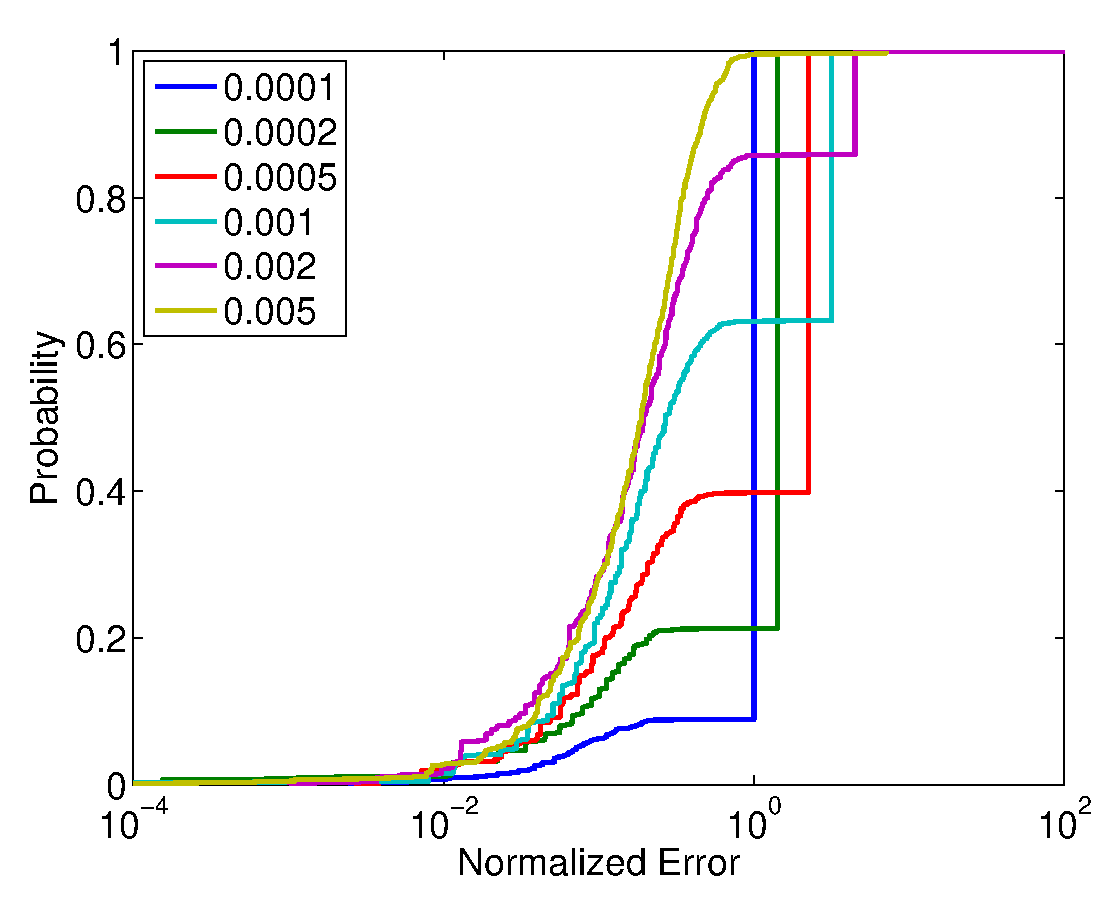
\includegraphics[width=3in]{NormalErrFig.eps}
\caption{Empirical distribution function of $\abs{\mu-\hmu_n}/\epsilon$ for example \eqref{exampleeq} with $\mu=\sigma=1$, $n_0=100$, $\kappa_{\max} = 3.2$, $\varepsilon=0.01$, and  $p=0.001, 0.002, 0.005, 0.01, 0.02, 0.05$ using the algorithm in Theorem \ref{mainadaptthm}. \label{normalerrfig}}
\end{figure}

Figure \ref{normalerrfig} shows the empirical distribution of the normalized error $\abs{\mu-\hmu_n}/\epsilon$, using $1000$ replications for a range of values of $p$.  As can be seen in this figure and in Table \ref{examptable}, the adaptive Monte Carlo method does poorly for very small values of $p$, which correspond to vary large values of the kurtosis.  However, even for values of the kurtosis above $\kappa_{\max}=3.2$ used in this example, the chance of meeting the error tolerance may be quite high.

\begin{table}
\caption{Kurtosis and probability of meeting the error tolerance for different values of $p$. \label{examptable}}
\[
\begin{array}{r|ccccccccccc}
p &   0.001 &    0.002 &    0.005 &     0.01 &     0.02 &     0.05 \\
\hline
\kappa &  998.00 &   498.00 &   198.01 &    98.01 &    48.02 &    18.05 \\
\hline
\Prob(\abs{\mu-\hmu_n} \le \varepsilon) &    8.70\% &    17.50\% &    39.20\% &    63.50\% &    86.40\% &    99.90\% \\
\end{array}
\]
\end{table}


\section{Questions}

Here are some questions that suggest themselves:

\begin{itemize}

\item Is this analysis above known already?  Is this the typical probabilistic setting?  Is it better to look at a randomized setting where one considers the expected value of the error?

\item Can this type of analysis be extended to randomized \emph{quasi-Monte Carlo} for finite dimension, $d$?  Infinite dimension?  In this latter case one needs some multilevel algorithm, but the specification of the levels perhaps could be deduced from the data.  One might also consider a case where the coordinate weights were not known a priori but needed to be estimated.

\item Is there already this kind of information-based complexity analysis where the number of operations is bounded above or below by the unknown scale of the problem (in this case the variance).  The IBC I know assumes that the scale is fixed, e.g., the function has variance one, norm one, etc.  Here we allow arbitrary scale, but do make assumptions on the nastiness (kurtosis).

\item Are there better inequalities than Chebyshev's inequality or the Berry-Esseen inequality that apply when $Z$ is the sum of i.i.d.\ random variables?  Some of the better known ones, like Hoeffding's inequality assume boundedness, which we cannot presume here.

\end{itemize}

\section*{Appendix of Useful Theorems}
\begin{theorem}[Chebyshev's Inequality] \label{Chebineqthm} Let $Z$ be any random variable with mean $\mu$ and variance $\sigma^2$.  Then for all $\alpha >0$, Chebyshev's inequality states that
\[
\Prob\left[\abs{Z-\mu} \ge \frac{\sigma}{\sqrt{\alpha}} \right] \le \alpha, \qquad \Prob\left[\abs{Z-\mu} < \frac{\sigma}{\sqrt{\alpha}} \right] \ge 1-\alpha.
\]
\end{theorem}
\begin{proof}To prove Chebyshev's inequality note that
\begin{equation*}
\sigma^2 = E[\abs{Z-\mu}^2] \ge \frac{\sigma^2}{\alpha} \Prob\left[\abs{Z-\mu} \ge \frac{\sigma}{\sqrt{\alpha}} \right],
\end{equation*}
and then divide both sides by $\sigma^2/\alpha$.
\end{proof}
The following theorem comes from \cite[Theorem 5.16, p. 168]{Pet95a}
\begin{theorem}[Non-uniform Berry-Esseen Inequality] \label{BE} Let $Y_1,\dots,Y_n$ be i.i.d.\ random variables.  Suppose that
\[
\mu=E(Y_i), \quad \var(Y_i)=\sigma^2>0, \quad \varrho=\frac{E\abs{Y_i - \mu}^3}{\sigma^3} < \infty.
\]
Then
\[
\abs{\Prob\left[\frac{1}{\sigma\sqrt{n}}\sum_{i=1}^{n}(Y_i-\mu)<x
\right]-\Phi(x)}\leq \frac{A \varrho}{\sqrt{n}}(1+\abs{x})^{-3}.
\] for all x,
where $\Phi$ is the cumulative distribution function of the standard normal random variable, and $A$ is some number satisfying $0.4097\leq A\leq 0.5600$.
\end{theorem}

\begin{theorem} \label{Varvarthm} Let $\hv_n$ be the sample variance as defined in \eqref{samplevar}.  It's variance is
\[
\var(\hv_n^2) = \frac{\sigma^4}{n} \left ( \kappa  - \frac{n-3}{n-1} \right),
\]
where $\kappa:= \kurt(g) = M_4(g)/\sigma^4(g)$ denotes the \emph{kurtosis}.
\end{theorem}
\begin{proof}The sample variance has mean $\sigma^2/n$.  To facilitate the derivation, let $Y_i=g(X_i) - \mu$.
\begin{align*}
\hv_n & =  \frac 1{n-1} \sum_{i=1}^n \left[Y_i- \left(\frac 1n \sum_{j=1}^n Y_j\right) \right]^2
=  \frac 1{n(n-1)}\left[ n \sum_{i=1}^n Y^2_i-  \sum_{j,k=1}^n Y_jY_k \right] \\
\hv_n^2 & = \frac 1{n^2(n-1)^2}\left[ n^2 \sum_{i,j=1}^n Y^2_i Y^2_j  - 2 n \sum_{i,j,k=1}^n Y^2_i Y_j Y_k +  \sum_{i,j,k,l=1}^n Y_iY_j Y_k Y_l\right] \\
E[ Y^2_i Y^2_j] & = \begin{cases} M_4, & i=j,\\
\sigma^4, & i \ne j,
\end{cases}\\
\sum_{i,j=1}^n E[Y^2_i Y^2_j]&= n M_4 + n(n-1)\sigma^4, \\
E[ Y^2_i Y_j Y_k] & = \begin{cases} M_4, & i=j=k,\\
\sigma^4, & i \ne j, j=k,\\
0, & j \ne k,
\end{cases} \\
\sum_{i,j,k=1}^n E[Y^2_i Y_j Y_k] &= nM_4  + n(n-1)\sigma^4 \\
E[ Y_i Y_j Y_k Y_l] & = \begin{cases} M_4, & i=j=k=l,\\
\sigma^4, & i, j, k, l \text{ have 2 distinct values},\\
0, & \text{otherwise},
\end{cases}\\
\sum_{i,j,k,l=1}^n E[Y_iY_j Y_k Y_l] &= n M_4 + 3n(n-1)\sigma^4 \\
E[\hv_n^2] & = \frac{ n^3[M_4 + (n-1)\sigma^4]  - 2 n^2 [M_4 + (n-1)\sigma^4] +  n[M_4 + 3(n-1)\sigma^4]} {n^2(n-1)^2} \\
& = \frac{ (n-1)M_4 + (n^2-2n+3)\sigma^4} {n(n-1)} \\
\var(\hv_n^2) & = E[\hv_n^2] - \left[E(\hv_n)\right]^2 = \frac{ (n-1)M_4 + (n^2-2n+3)\sigma^4} {n(n-1)} -\sigma^4\\
& = \frac{(n-1)M_4 + (-n+3)\sigma^4} {n(n-1)}= \frac{1}{n} \left ( M_4 - \frac{n-3}{n-1} \sigma^4 \right) = \frac{\sigma^4}{n} \left ( \kappa  - \frac{n-3}{n-1} \right).
\end{align*}
\end{proof}
\begin{theorem}[Single tailed Cantelli's inequality]\label{Can}
Let $Z$ be any random variable with mean $\mu$ and finite variance $\sigma^2$.  For any $a\geq 0$, it
follows that:
\[
\Prob[Z-\mu \geq a]\leq \frac{\sigma^2}{a^2+\sigma^2}.
\]
\end{theorem}
\begin{proof}Define the random variable
\[ S=\sign(Z - \mu - a) = \begin{cases} 1, & Z - \mu \geq a,\\ -1, & Z - \mu <a. \end{cases}
\]
From conditional probability it is known that
\begin{align*}
\sigma^2 &= \var(Z-\mu)=E[\var(Z-\mu|S)]+\var[E(Z-\mu|S)] \\
&\geq\var[E(Z-\mu|S)]= E[\{E(Z-\mu|S)\}^2]-[E\{E(Z-\mu|S)\}]^2 =  E[\{E(Z-\mu|S)\}^2]
\end{align*}
Since $E(Z-\mu)=0$, it follows that
\begin{equation*}
0= E[E(Z-\mu|S)]=E(X|S=1)\Prob(Z - \mu \geq a)+E(X|S=-1)\Prob(Z - \mu < a).
\end{equation*}
Also, it is clear that $E(Z - \mu|S=1) \ge a$, which implies that
\begin{equation*}
[E(Z - \mu|S=-1)]^2=\left[\frac{E(Z - \mu|S=1)\Prob(Z - \mu \geq a)}{\Prob(Z - \mu < a)}\right]^2\geq \left[\frac{a\Prob(Z - \mu \geq a)}{\Prob(Z - \mu < a)}\right]^2
\end{equation*}
Combining these results together yields
\begin{align*}
\sigma^2 & \ge E[\{E(Z-\mu|S)\}^2]\\
& =\{E(Z-\mu|S=1)\}^2 \Prob(Z - \mu \geq a) + \{E(Z-\mu|S=-1)\}^2 \Prob(Z - \mu < a) \\
& \ge a^2 \Prob(Z - \mu \geq a) + \left[\frac{a\Prob(Z - \mu \geq a)}{\Prob(Z - \mu < a)}\right]^2 \Prob(Z - \mu < a) \\
&= a^2 \left[\frac{ \Prob(Z - \mu \geq a)}{\Prob(Z - \mu < a)}\right] = a^2 \left[\frac{ \Prob(Z - \mu \geq a)}{1  - \Prob(Z - \mu \ge a)}\right]
\end{align*}
Solving this inequality for $\Prob(Z - \mu \geq a)$ completes the proof.
\end{proof}

\begin{prop}\label{propCant} Let $\hv_n$ be the sample variance of a function $g$ as defined in \eqref{samplevar}, and let $\kappa=\kurt(g)$.  Then
\begin{subequations} \label{sampvarbd}
\begin{gather}\label{sampvarup}
\Prob\left[\hv_n < \sigma^2 \left\{1 + \sqrt{\left ( \kappa  - \frac{n-3}{n-1}\right)\left(\frac{1-\alpha}{\alpha n}\right)}\right\} \right] \ge 1 - \alpha, \\
\label{sampvarlo}
\Prob\left[\hv_n > \sigma^2 \left\{1 - \sqrt{\left ( \kappa  - \frac{n-3}{n-1}\right)\left(\frac{1-\alpha}{\alpha n}\right)}\right\} \right] \ge 1 - \alpha.
\end{gather}
\end{subequations}
\end{prop}
\begin{proof}Choosing
$$a=\sigma^2\sqrt{\left(\kappa-\frac{n-3}{n-1}\right)\left(\frac{1-\alpha}{\alpha n}\right)} >0,
$$
we know from Cantelli's inequality (Theorem \ref{Can})  that
$$\Prob[\hv_n-\sigma^2 \geq
a]\leq\frac{\var(\hv_n)}{a^2+\var(\hv_n)}$$
\begin{align*}
\Prob\left[\hv_n-\sigma^2 \geq
\sigma^2\sqrt{\left(\kappa-\frac{n-3}{n-1}\right)\left(\frac{1-\alpha}{\alpha n}\right)} \right] & = \Prob\left[\hv_n-\sigma^2 \geq
a \right]\\
& \leq\frac{\var(\hv_n)}{a^2+\var(\hv_n)}\\
&= \frac{\frac{\sigma^4}{n}\left(\kappa - \frac{n-3}{n-1}\right)}{\frac{\sigma^4}{n}\left(\kappa - \frac{n-3}{n-1}\right)\left(\frac{1-\alpha}{\alpha}\right)+\frac{\sigma^4}{n}\left(\kappa - \frac{n-3}{n-1}\right)} \\
&=\frac{1}{\left(\frac{1-\alpha}{\alpha}\right)+1}=\alpha.
\end{align*}
Then \eqref{sampvarup} follows directly.  By a similar argument.
\begin{align*}
\Prob\left[\hv_n-\sigma^2 \le
- \sigma^2\sqrt{\left(\kappa-\frac{n-3}{n-1}\right)\left(\frac{1-\alpha}{\alpha n}\right)} \right] & = \Prob\left[\hv_n-\sigma^2 \le -a \right]\\
& = \Prob\left[(-\hv_n)-(-\sigma^2) \ge a \right]\\& \leq\frac{\var(-\hv_n)}{a^2+\var(-\hv_n)}= \frac{\var(\hv_n)}{a^2+\var(\hv_n)}\\
&= \frac{\frac{\sigma^4}{n}\left(\kappa - \frac{n-3}{n-1}\right)}{\frac{\sigma^4}{n}\left(\kappa - \frac{n-3}{n-1}\right)\left(\frac{1-\alpha}{\alpha}\right)+\frac{\sigma^4}{n}\left(\kappa - \frac{n-3}{n-1}\right)} \\
&=\frac{1}{\left(\frac{1-\alpha}{\alpha}\right)+1}=\alpha.
\end{align*}
Thus, \eqref{sampvarlo} follows as well.
\end{proof}

\bibliographystyle{spbasic}
\bibliography{FJH21,FJHown21}
\end{document}
